\documentclass[red]{beamer}

\mode<presentation>{
\usetheme{Goettingen}
\usecolortheme{default}
}

\setbeamertemplate{itemize/enumerate body begin}{\footnotesize}
\setbeamertemplate{itemize/enumerate subbody begin}{\scriptsize}
\usepackage{CJK}
\usepackage{graphicx}
\usepackage{amsmath, amsopn}
\usepackage[english]{babel}
\usepackage[latin1]{inputenc}
\usepackage{url}
\usepackage{color}
\usepackage{times}
\usepackage{xcolor}
\usepackage{listings}
\lstset{
language=bash,
keywordstyle=\color{blue!70}\bfseries,
basicstyle=\ttfamily\scriptsize,
commentstyle=\ttfamily,
showspaces=false,
showstringspace=false,
showtabs=false,
frame=no,
rulesepcolor=\color{red!20!green!20!blue!20},
breaklines=true}
\title[BI296-Lec02]{\tiny{BI296: Linux and Shell Programming}\\
\Large{Lecture 02: Linux Command Line}}
\author[Maoying Wu]{Maoying,Wu\\
{\scriptsize ricket.woo@gmail.com}}
\institute[CBB] % (optional, but mostly needed)
{
  \inst{}
  Dept. of Bioinformatics \& Biostatistics\\
  Shanghai Jiao Tong University
}
\date{Spring, 2017}

\AtBeginSubsection[]
{
  \begin{frame}<beamer>{Next we will talk about ...}
    \tableofcontents[currentsection,currentsubsection]
  \end{frame}
}

\newcommand{\tabincell}[2]{\begin{tabular}{@{}#1@{}}#2\end{tabular}}

\begin{document}
\begin{CJK*}{UTF8}{gbsn}
\frame{\titlepage}

\begin{frame}
\frametitle{Quick Recaps}
\begin{itemize}
	\item Decimal/Binary/Octal/Hexadecimal numbers and their cross-conversion
	\item Original digit (源码), One's complement(反码), Two's complement(补码)
	\item bit, byte, kilobyte, megabyte, gigabyte, terabyte, ...
	\item Richard Stallman, GNU, Free and Open-source, FSF
	\item Linus Torvalds, Unix, Linux, Tux
	\item Middleware of hardware and user, utilities 
\end{itemize}
\end{frame}


\begin{frame}[containsverbatim]
\frametitle{Some Basic Commands}
\begin{itemize}
	\item \textbf{System information}: {\lstinline{uname, uptime, arch, nproc, hostname, hostid}}
	\item \textbf{User management}: {\lstinline{id, user, passwd, mkpasswd, useradd, userdel, groupadd, groupdel, groupmems}}
	\item \textbf{Environment-related}: {\lstinline{env, export}}
	\item \textbf{File system}: {\lstinline{ls, file, cd, mkdir, rmdir, rm, mv, cp, stat}}
	\item \textbf{Help information}: {\lstinline{man, info, whatis}}
	\item \textbf{Process control}: {\lstinline{ps, pstree, fg, bg, jobs, nohup}}
	\item \textbf{File searching}: {\lstinline{locate, whereis, which, find}}
\end{itemize}
\end{frame}


\begin{frame}[fragile,containsverbatim]
\frametitle{Print system information}
\begin{table}[ht]
\scriptsize
\renewcommand\arraystretch{1.6}
\begin{tabular}{ll}
\hline
\textbf{Command} & \textbf{Description}\\
\hline
\texttt{uname -a} & print all information\\
\texttt{uname -s} & print the kernel name\\
\texttt{uname -n} & print the network node hostname\\
\texttt{uname -r} & print the kernel release\\
\texttt{uname -m} & print the machine hardware name\\
\texttt{uname -p} & print the processor type or "unknown"\\
\texttt{uname -i} & print the hardware platform or "unknown"\\
\texttt{uname -o} & print the operating system\\
\hline
\end{tabular}
\end{table}
\begin{lstlisting}[basicstyle=\tiny]
[bio@localhost ~]$ uname -a
Linux localhost.localdomain 3.10.0-327.el7.x86_64 #1 SMP Fri Nov 20 11:12:42 CST 2015 x86_64 x86_64 x86_64 GNU/Linux
\end{lstlisting}
\end{frame}


\begin{frame}[containsverbatim]
\frametitle{The other system-context commands}
\begin{itemize}
	\item \lstinline{date}: print or set the system date and time.
	\item \lstinline{arch}: print machine hardware name.
	\item \lstinline{nproc}: print the number of processing units available.
	\item \lstinline{hostname}: show or set the system's host name.
	\item \lstinline{hostid}: print the numeric identifier for the current host.
	\item \lstinline{uptime}: tell how long the system has been running.
\end{itemize}
\end{frame}


\begin{frame}[containsverbatim]
\frametitle{Print something}
\begin{itemize}
	\item \lstinline{echo "I am genius!"  # using double quotes}
	\item \lstinline{echo 'I am genius!' # using single quotes}
	\item \lstinline{echo I am genius! # no quotes}
	\item \lstinline{echo $SHELL # print environment variable}
	\item \lstinline{echo $HOSTNAME # print environment variable}
	\item \lstinline{echo "$HOSTNAME is running under $SHELL"}
\end{itemize}
\begin{figure}[ht]
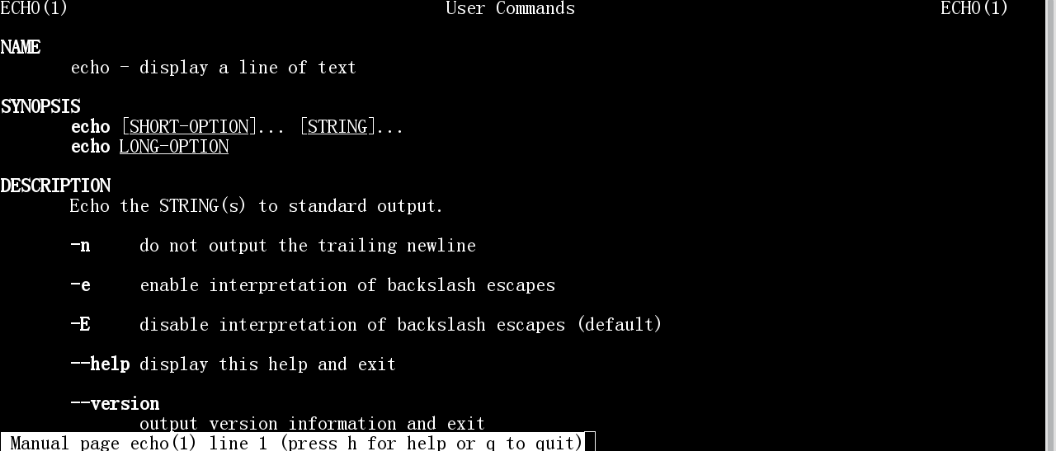
\includegraphics[width=0.80\textwidth]{images/echo.png}
\end{figure}
\end{frame}

\begin{frame}[fragile,containsverbatim]
\frametitle{Formatting output}
\lstinline{printf}
\begin{lstlisting}[basicstyle=\ttfamily\tiny]
[bio@localhost ~]$ printf "UserName\tUserID\t\tGroupID\t\tDescription\n"
UserName	UserID		GroupID		Description
[bio@localhost ~]$ printf "The cost is \v%-5.2f dollars\n" 12.5 
The cost is 
            12.50 dollars
\end{lstlisting}
\begin{figure}[ht]
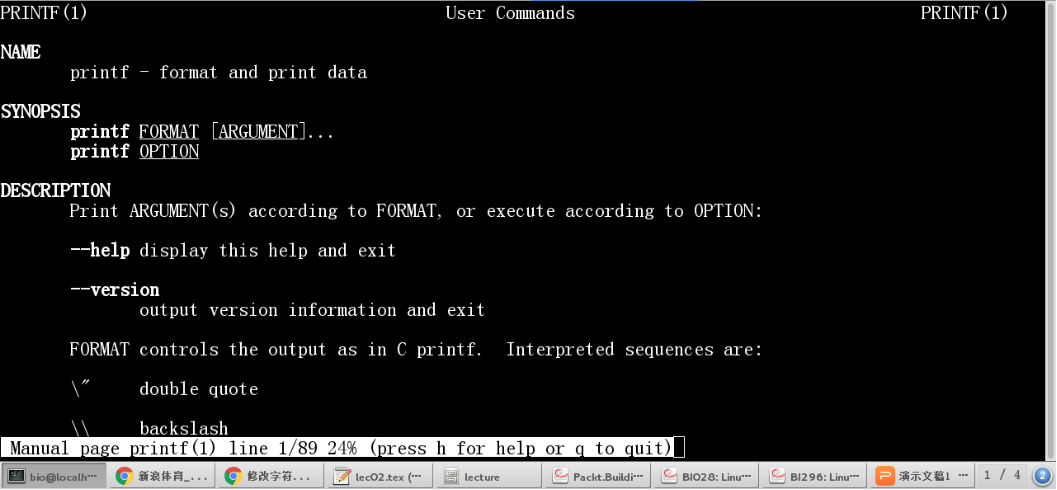
\includegraphics[width=0.80\textwidth]{images/printf.png}
\end{figure}
\end{frame}

\begin{frame}[fragile,containsverbatim]
\frametitle{Getting help}
\begin{table}[ht]
\scriptsize
\renewcommand\arraystretch{1.6}
\begin{tabular}{ll}
\hline
\textbf{Category} & \textbf{Example}\\
\hline
\texttt{CMD -h,--help} & \texttt{ls -h}\\
\texttt{man} & \texttt{man 1 ls}\\
\texttt{info} & \texttt{info ls}\\
\texttt{whatis} & \texttt{whatis ls}\\
\hline
\end{tabular}
\end{table}
\begin{figure}[ht]
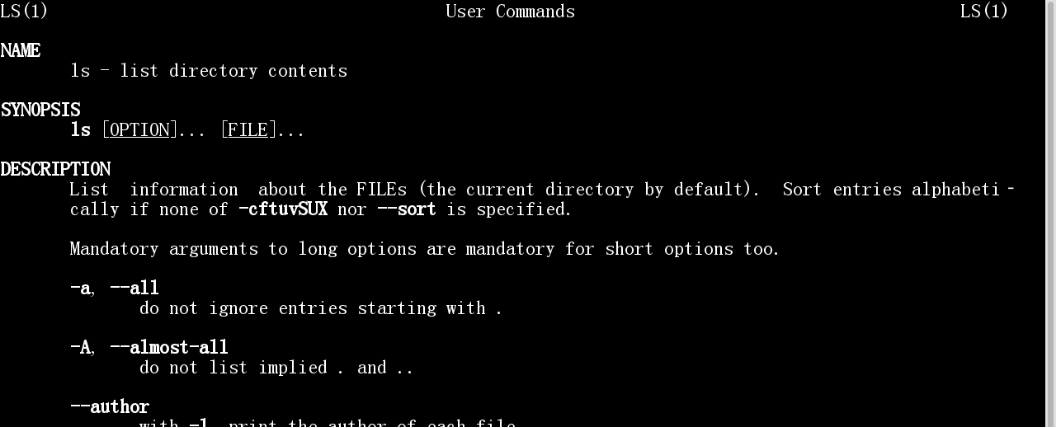
\includegraphics[width=0.80\textwidth]{images/ls.png}
\end{figure}
\end{frame}


\begin{frame}
\frametitle{man}
\begin{figure}
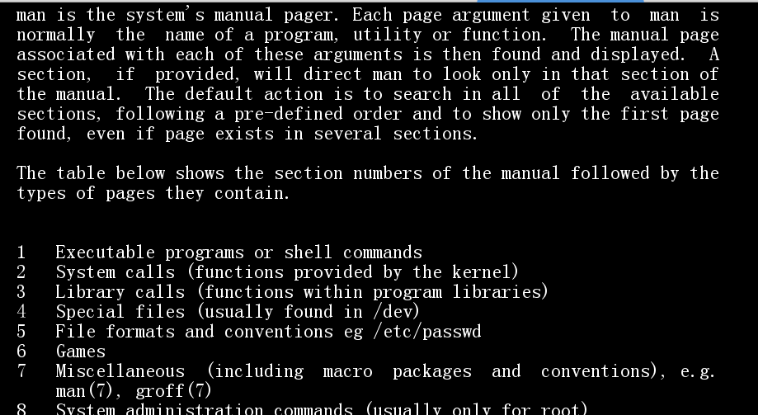
\includegraphics[width=0.80\textwidth]{images/man.png}
\end{figure}
\end{frame}


\begin{frame}
\frametitle{info}
\begin{figure}
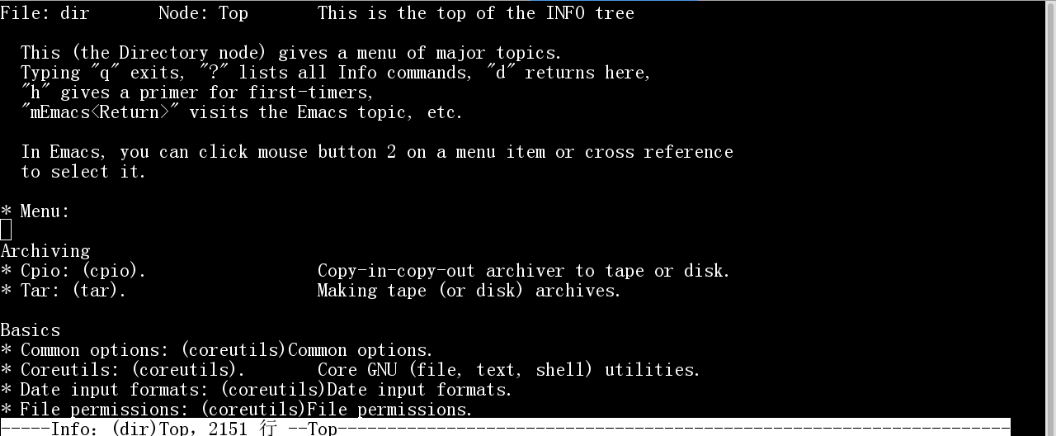
\includegraphics[width=0.80\textwidth]{images/info.png}
\end{figure}
\end{frame}

\section{Files}

\begin{frame}[containsverbatim]
\frametitle{File types}
\begin{itemize}
	\item \lstinline{ls -l /dev/sda1}
	\item \lstinline{file /dev/sda1}
\end{itemize}
\begin{table}[ht]
\scriptsize
\renewcommand\arraystretch{1.6}
\begin{tabular}{lll}
\hline
\textbf{File type} & \textbf{Description} & \textbf{Example} \\
\hline
Regular file (-) & Plain data file & /etc/passwd, /bin/bash \\
Directory (d)& A directory entry & /usr\\
Block special file (b) & Block device & /dev/sda1 \\
Character special file (c) & Character device & /dev/null \\
FIFO (p) & Named pipe & /run/systemd/initctl/fifo \\
Socket (s) & /tmp/mysqld.sock \\
Symbolic link (l) & Symbolic link & /usr/lib64/libc.so.6 \\
\hline
\end{tabular}
\end{table}

\begin{lstlisting}[language=bash,basicstyle=\ttfamily\tiny,]
[bio@localhost ~]$ file /usr/lib64/libc-2.17.so
/usr/lib64/libc-2.17.so: ELF 64-bit LSB shared object, x86-64, version 1 (GNU/Linux), dynamically linked (uses shared libs), BuildID[sha1]=53c0918c85fa9cc08d2b57e76467631ab07554ae, for GNU/Linux 2.6.32, not stripped
\end{lstlisting}

\end{frame}


\begin{frame}
\frametitle{File permissions}
\begin{itemize}
	\item Four access levels
	\begin{itemize}	\scriptsize
		\item user(u): The user that owns the file
		\item group(g): The group that owns the file
		\item others(o): The others except the owner and group
		\item all(a): all the users
	\end{itemize}
	\item Three permissions
	\begin{itemize}	\scriptsize
		\item Read(r): Read content of a file or list content of a directory
		\item Write(w): Change content of a file or create/delete files in a
					directory
		\item Execute(x): Execute files as a program or use directory as active 
				directory
	\end{itemize}
	\item Special file permission
	\begin{itemize}	\scriptsize
		\item Setuid, setgid(s): special permissions for executable files. 
			Any user who runs that executable file assumes the user ID of the 
			owner/group of the file.
		\item Sticky-bit(t): special permission for public directories. 
	\end{itemize}
\end{itemize}
\begin{figure}[ht]
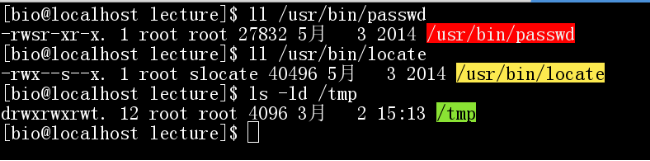
\includegraphics[width=0.80\textwidth]{images/setuid.png}
\end{figure}
\end{frame}

\begin{frame}
\frametitle{Directory permissions}
\begin{table}[ht]
\scriptsize
\renewcommand\arraystretch{1.6}
\begin{tabular}{ll}
\hline
\textbf{Symbol} & \textbf{Description}\\
\hline
\texttt{r}	& List files in the directory.\\
\hline
\texttt{w} & Add or remove files/directories/links in the directory.\\
\hline
\texttt{x} & \tabincell{l}{Open/execute files in the directory, \\ change to the directory and subdirectories.}\\
\hline
\end{tabular}
\end{table}
\end{frame}


\begin{frame}[fragile,containsverbatim]
\frametitle{Change the permission of a file}
\begin{table}[ht]
\scriptsize
\renewcommand\arraystretch{1.6}
\begin{tabular}{ll}
\hline
\textbf{Command} & \textbf{Description}\\
\hline
\texttt{ls -l filename} & list the properties of a file\\
\texttt{chown bio:bio filename} & change the owner/group of a file\\
\texttt{chgrp bio filename} & change the group of a file\\
\texttt{chmod 755 filename} & change the mode/permission of a file\\
\texttt{chmod u+w filename} & add write permission for the owner\\
\texttt{chattr -A filename} & change the attribute of a file\\
\texttt{lsattr filename} & list the attributes of a file\\
\hline
\end{tabular}
\end{table}
\begin{figure}[ht]
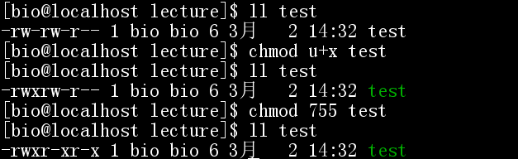
\includegraphics[width=0.80\textwidth]{images/chmod.png}
\end{figure}
\end{frame}

\begin{frame}[containsverbatim]
\frametitle{\texttt{umask}}
\begin{itemize}
	\item By default, the system sets the permission on a text file 
		to 666, and to 777 on a directory or executable file.
	\item The value assigned by the \lstinline{umask} command is 
		subtracted from the default.
	\item \lstinline{umask 022} command denies write permission for 
		group and others.
	\item Usually the \texttt{root} and a normal user has different 
		\lstinline{umask} strategies. Why?
\end{itemize}
\end{frame}

\begin{frame}[fragile,containsverbatim]
\frametitle{Display file status}
\lstinline{stat filename}
\begin{figure}[ht]
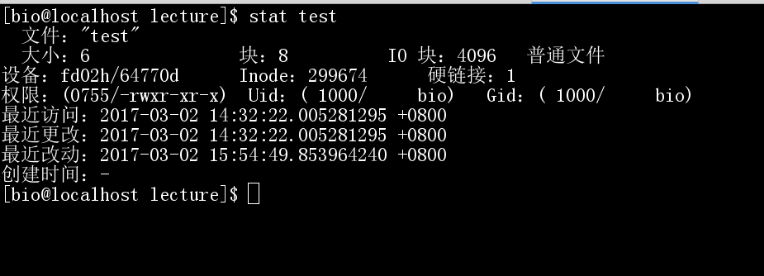
\includegraphics[width=0.80\textwidth]{images/stat.png}
\end{figure}
\begin{itemize}
	\item \texttt{mtime}: last time the file content was modified, \lstinline{ls -l}
	\item \texttt{ctime}: last time of file status modification, \lstinline{ls -lc}
	\item \texttt{atime}: last access time, \lstinline{ls -lu}
	\item \texttt{crtime}: creation time, \lstinline{stat --printf '%n: created %w\n'}
\end{itemize}
\end{frame}

\begin{frame}[containsverbatim]
\frametitle{Display file contents}
\begin{itemize}
	\item Display entire file
	\begin{itemize}
		\item \lstinline{cat, tac /etc/passwd}
		\item \lstinline{less, more /etc/passwd}
		\item \lstinline{nl /etc/passwd}
		\item \lstinline{od /etc/passwd}
		\item \lstinline{base64 /etc/passwd}
	\end{itemize}
	\item Display parts of file
	\begin{itemize}
		\item \lstinline{head /etc/passwd}
		\item \lstinline{tail /etc/passwd}
		\item \lstinline{split -d -n 2 /etc/passwd passwd.}
	\end{itemize}
	\item Formatting file contents
	\begin{itemize}
		\item \lstinline{fmt }
		\item \lstinline{pr -o 5 /etc/passwd}
		\item \lstinline{fold -w 20 /etc/passwd}
	\end{itemize}
\end{itemize}
\end{frame}


\begin{frame}[containsverbatim]
\frametitle{The other commands relating to file and directory}
\begin{itemize}
	\item Directory listing: \lstinline{ls, dir}
	\item Basic operations: \lstinline{cp, dd, mv, rm}
	\item Directory operations: \lstinline{mkdir, rmdir, cp, mv}
	\item Changing file attributes: \lstinline{chgrp, chmod, chown, touch}
	\item Summarizing files: \lstinline{wc, sum, md5sum}
	\item Sorted files: \lstinline{sort, uniq, comm}
	\item Operating on fields: \lstinline{cut, paste, join}
	\item Operating on characters: \lstinline{tr, expand}
	\item Creating link file: \lstinline{ln}
\end{itemize}
\end{frame}


\begin{frame}[containsverbatim]
\frametitle{\texttt{ln}: creating link file}
\begin{itemize}
	\item \lstinline{ln a b}: create hard link \texttt{b} for \texttt{a}
	\item \lstinline{ln -s a b}: create symbolic link \texttt{b} for \texttt{a}
	\item Can you create a hard link for a directory? symbolic link?
	\item Can you create a hard link between different operating systems? symbolic link?
\end{itemize}
\end{frame}

\begin{frame}[containsverbatim]
\frametitle{Exercise (1)}
\begin{enumerate}
	\item What is the difference between \lstinline{man 1 printf} and 
			\lstinline{man 3 printf}?
	\item We have known that the command \lstinline{tree} can print out 
		the directory tree. How to set the output level to be 2?
	\item Compare \lstinline{ls -a} and \lstinline{ls -A}. Can you find 
		what this option "-a" is able to do?
	\item What is the difference among commands \lstinline{cat, less} and
		\lstinline{more} to view the content of a regular file?
	\item What is the usage of the command \lstinline{umask}? List the
		possible distinctions between dealing with files and with 
		directories?
	\item Tell the difference between hard link and symbolic link? If I
			would like to use \lstinline{ln} to create a hard link file2 for
			file1, what should I do? If we delete file1, what will happen 
			to file2? How about symbolic link?
\end{enumerate}
\end{frame}

\begin{frame}[containsverbatim]
\frametitle{Exercise (2)}
\begin{enumerate}
	\item What is the difference between \lstinline{whoami} and \lstinline{who am i}?
	\item What does \lstinline{chmod 735 file1} do? If we want to prevent a
		folder \texttt{new} from being accessed by all the user except the
		owner, what should we do?
	\item How to create a multiple-level directory \texttt{/tmp/a/b/c/d} using
		\lstinline{mkdir} in exactly one line command?
	\item Tell what the following commands can do for you.
	\begin{itemize}
		\item \lstinline{chmod u+w file2}
		\item \lstinline{chmod a-x file2}
		\item \lstinline{chmod 644 file2}
		\item \lstinline{chmod o=rwx file2}
	\end{itemize}
\end{enumerate}
\end{frame}

\section{User-Related Commands}

\begin{frame}
\frametitle{Users}
\begin{itemize}
	\item Each user has a unique username and userID
	\item A user can belong to more than one group
	\item All the users are stored in the file \texttt{/etc/passwd}
	\item The encrypted password for each user is stored in the file 
		\texttt{/etc/shadow}
	\item The user can be added using \lstinline{useradd} command, and 
		modified by \lstinline{usermod}, and deleted by \lstinline{userdel}
	\item For each user, the private environment is defined by the file 
		\texttt{~/.bashrc} and the common environment is defined in the 
		file \texttt{/etc/bashrc} and \texttt{/etc/profile}
	\item The default settings for \lstinline{useradd} is defined in the 
		file \texttt{/etc/default/useradd}.
\end{itemize}
\begin{figure}[ht]
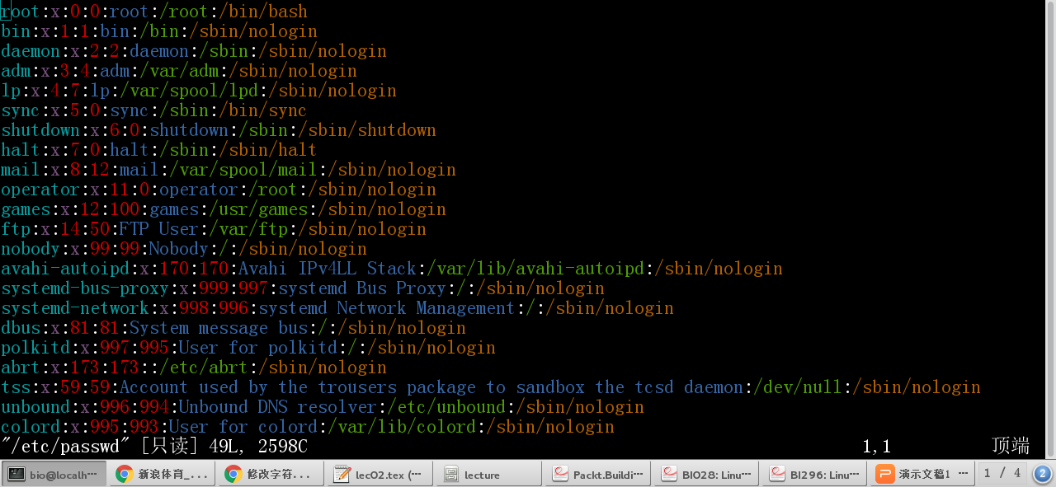
\includegraphics[width=0.80\textwidth]{images/passwd.png}
\end{figure}
\end{frame}


\begin{frame}
\frametitle{Output of user information}
\begin{itemize}
	\item \lstinline{id}: print real and effective user and group IDs.
	\item \lstinline{logname}: print user's login name.
	\item \lstinline{whoami}: print effective user id.
	\item \lstinline{groups}: print the groups the user is in
	\item \lstinline{users}: print the user names of users currently logged 
		in to the current host.
	\item \lstinline{who}: show who is logged in.
	\item \lstinline{w}: Show  who is logged on and what they are doing.
\end{itemize}
\end{frame}


\begin{frame}[containsverbatim]
\frametitle{Exercise}
Have a look at the manual page of the command \lstinline{groupmems} and the 
configuration file \texttt{/etc/sudoers}.
\begin{enumerate}
	\item Log in to the system as the root;
	\item Enable the group \texttt{wheel} has the \lstinline{sudo} privilege;
	\item Recruit the user 'bio' into the group \texttt{wheel};
	\item Use command \lstinline{id} to confirm whether the above job work;
	\item Try run \lstinline{sudo su - root} to check whether the \lstinline{sudo}
		privilege work for user \texttt{bio}.
\end{enumerate}
\end{frame}

\section{Process control}

\begin{frame}[containsverbatim]
\frametitle{Process control (1)}
\begin{table}[ht]
\scriptsize
\renewcommand\arraystretch{1.6}
\begin{tabular}{ll}
\hline
\textbf{Command} & \textbf{Description}\\
\hline
\texttt{CTRL+z} & Stop (interrupt) a foreground process.\\
\texttt{CTRL+c} & Kill a foreground job.\\
\texttt{ps} & list the running processes.\\
\texttt{pstree} & print the process tree.\\
\texttt{fg} & run the suspended job in foreground.\\
\texttt{bg} & Run the suspended job in background.\\
\texttt{jobs} & List the background or suspended jobs.\\
\texttt{CMD \&} & place the job in the background.\\
\texttt{nohup CMD \&} & run in the background.\\
\texttt{kill} & Kill a running process or suspended jobs.\\
  
\hline
\end{tabular}
\end{table}
\end{frame}

\begin{frame}[containsverbatim]
\frametitle{Process control (2)}
\begin{enumerate}
	\item Type in the command \lstinline{yes I am genius}
	\item Press \texttt{CTRL+z} to suspend the running process
	\item Use \lstinline{jobs} to look through the suspended or background
		processes
	\item Use \lstinline{fg %job-id} to bring the process to foreground, or
	\item Use \lstinline{bg %job-id} to run the job in background, or
	\item use \lstinline{kill %job-id} to kill the process
\end{enumerate}
\end{frame}


\begin{frame}[containsverbatim]
\frametitle{Standard streams}
\begin{itemize}
	\item Standard Input (stdin: 0)
	\begin{itemize}
		\item Generally it is a keyboard.
	\end{itemize}
	\item Standard Output (stdout: 1)
	\begin{itemize}
		\item Generally it is the terminal or the printer. 
	\end{itemize}
	\item Standard Error (stderr: 2)
	\begin{itemize}
		\item Generally it is the terminal.
	\end{itemize}
\end{itemize}
\end{frame}


\begin{frame}[containsverbatim]
\frametitle{Piping}
\begin{itemize}
	\item The STDOUT of a command acts as the STDIN of the next command.
	\item \textbf{Examples}
	\begin{itemize}
		\item \lstinline{cat /etc/paswd | wc -l}\\count the number of lines in the file.
		\item \lstinline{cat /etc/passwd | grep mysql}\\see if the user exists.
		\item \lstinline{ls -l /dev | less}\\view the content as stream
		\item \lstinline{gunzip file.tar.gz | tar xvf -}\\uncompress the .tar.gz file.
	\end{itemize}
\end{itemize}
\end{frame}


\begin{frame}[containsverbatim]
\frametitle{Redirection}
\begin{itemize}
	\item STDIN Redirection
	\begin{itemize}
		\item \lstinline{cat 0< /etc/passwd}
		\item \lstinline{cat < /etc/passwd}
	\end{itemize}
	\item STDOUT Redirection
	\begin{itemize}
		\item \lstinline{ls -l > filelist.log}\\redirect the output to the file
		\item \lstinline{ls -l 1> filelist.log}\\redirect the stdout to the file
		\item \lstinline{ls -l >> filelist.log}\\append the stdout to the file
	\end{itemize}
	\item STDERR Redirection
	\begin{itemize}
		\item \lstinline{ls -z 2> err.log}\\redirect the stderr to the file
		\item \lstinline{ls -z 1> run.log 2>&1}\\redirect both the stdout and stderr to the file
		\item \lstinline{ls -z 2>/dev/null}\\suppress the output of the stderr
	\end{itemize}
\end{itemize}
\end{frame}


\begin{frame}[containsverbatim]
\frametitle{Disk usage}
\begin{itemize}
	\item \lstinline{fdisk -l}\\manipulate disk partition table.
	\item \lstinline{df -h}\\report file system disk space usage.
	\begin{lstlisting}[basicstyle=\ttfamily\tiny]
Filesystem                   Size  Used Avail Use% Mounted on
/dev/sda2                     50G   35G   16G  69% /
/dev/sda3                    177G  106G   72G  60% /home
/dev/sda1                    497M  158M  340M  32% /boot
	\end{lstlisting}
	\item \lstinline{du -sh /home/bio}\\estimate file space usage.
	\begin{lstlisting}[basicstyle=\ttfamily\tiny]
102G	/home/bio
	\end{lstlisting}
	\item \lstinline{stat -f /}\\display system status.
	\begin{lstlisting}[basicstyle=\ttfamily\tiny]
  File: "/"
    ID: fd0000000000 Namelen: 255     Type: xfs
Block size: 4096       Fundamental block size: 4096
Blocks: Total: 13100800   Free: 4125851    Available: 4125851
Inodes: Total: 52428800   Free: 51628882
	\end{lstlisting}
\end{itemize}
\end{frame}


\begin{frame}[containsverbatim]
\frametitle{Exercises}
The command \lstinline{ls -i} can list the inode number of the requested file.
\begin{enumerate}
	\item Use \lstinline{echo} and redirection to create a new file;
	\item Use \lstinline{cp} to create a new copy of the above file;
	\item Use \lstinline{mv} to create a new file of the above file;
	\item Use \lstinline{ln} to create a hard link of the above file;
	\item Use \lstinline{ln -s} to create a symbolic link of the above file;
	\item Use \lstinline{ls -i} to check whether the files have the same index node.
	\item Tell the difference among \lstinline{cp, mv, ln, ln -s}.
\end{enumerate}
\end{frame}


\begin{frame}[containsverbatim]
\frametitle{Bring-home Exercises}
\begin{enumerate}
\scriptsize
	\item A project requires that a set of users should share a directory 
		so that all of them can create/modify/remove the files/subdirectories 
		beneath the directory.
		\vskip 1pt
		For the sake of security, the directory cannot be accessed by the 
		other users.
		\vskip 1pt
		Can you figure out a solution? You should provide both your idea and 
		a practical example.
	\vskip 2em
	\item The command \lstinline{man hier} will output the directory tree 
		of the system as well as what they will host. Write a short essay 
		to illustrate the directory tree of the Linux system.
	\vskip 2em
	\item \lstinline{vim} is a very popular text editor under Linux system. 
		Please have a look at the tutorial we provided in the course webpage. 
\end{enumerate}  
\end{frame}


\end{CJK*}
\end{document}
